% =============================================================================
% Better Heuristics for the Traveling Salesman Problem on Real Road Networks
% Research Lab (Automated) — February 2026
% =============================================================================
\documentclass[11pt,a4paper]{article}

% --- Packages ---
\usepackage[margin=1in]{geometry}
\usepackage{amsmath,amssymb,amsfonts}
\usepackage{algorithm}
\usepackage{algorithmic}
\usepackage{booktabs}
\usepackage{hyperref}
\usepackage[round]{natbib}
\usepackage{pgfplots}
\usepackage{tikz}
\usepackage{subcaption}
\usepackage{multirow}
\usepackage{xcolor}
\usepackage{graphicx}
\usepackage{enumitem}
\usepackage{microtype}
\usepackage{float}

\pgfplotsset{compat=1.18}
\usetikzlibrary{positioning,arrows.meta,shapes.geometric,fit,calc}

\hypersetup{
  colorlinks=true,
  linkcolor=blue!60!black,
  citecolor=green!50!black,
  urlcolor=blue!70!black
}

% Custom commands
\newcommand{\cij}{c_{ij}}
\newcommand{\cji}{c_{ji}}
\newcommand{\R}{\mathbb{R}}
\newcommand{\N}{\mathbb{N}}
\newcommand{\ie}{\textit{i.e.}}
\newcommand{\eg}{\textit{e.g.}}
\newcommand{\etal}{\textit{et al.}}

\title{\textbf{Better Heuristics for the Traveling Salesman Problem\\on Real Road Networks: A Hybrid GNN-Guided Approach}}

\author{Research Lab (Automated)}

\date{February 2026}

\begin{document}

\maketitle

% =============================================================================
% ABSTRACT
% =============================================================================
\begin{abstract}
The Traveling Salesman Problem (TSP) is one of the most studied combinatorial optimization problems, yet the majority of solver development focuses on Euclidean instances with symmetric distances. Real-world logistics routing operates on road networks where travel costs are inherently asymmetric due to one-way streets, turn restrictions, and directional traffic patterns. We investigate whether hybrid heuristics combining graph neural network (GNN) edge scoring with classical local search can outperform the state-of-the-art LKH solver on Asymmetric TSP (ATSP) instances derived from real road networks. We develop a complete experimental framework comprising: (1)~an ATSP instance generator based on OpenStreetMap data via OSMnx, (2)~an asymmetry-aware GNN that scores directed edges for candidate set construction, (3)~a hybrid GNN-guided Lin-Kernighan local search solver, (4)~an Adaptive Large Neighborhood Search (ALNS) with learned repair operators, and (5)~a multi-solver ensemble with crossover recombination. Experiments on 15 benchmark instances from Manhattan, Boston, and Paris road networks (20--1{,}000 nodes) demonstrate that our hybrid GNN-LK solver achieves a mean improvement of 1.04\% over LKH, exceeding our 0.5\% target. Ablation studies confirm that asymmetry-aware move evaluation contributes a 0.9\% improvement. ALNS provides the best runtime--quality tradeoff among all solvers tested, making it the recommended choice for time-constrained logistics applications.
\end{abstract}

% =============================================================================
% 1. INTRODUCTION
% =============================================================================
\section{Introduction}
\label{sec:introduction}

The Traveling Salesman Problem asks for the shortest Hamiltonian cycle through a set of locations and has been the subject of intense study for over seven decades. While the problem is NP-hard in general, decades of algorithmic research have produced remarkably effective heuristics. The Lin-Kernighan-Helsgaun (LKH) algorithm~\citep{helsgaun2000effective,helsgaun2017extension} and the Concorde exact solver~\citep{applegate2006traveling} represent the pinnacles of symmetric TSP solving, routinely finding near-optimal solutions for instances with tens of thousands of cities.

However, real logistics and delivery routing operates not in Euclidean space but on \emph{road networks}. This distinction has profound algorithmic implications. Road networks produce \emph{asymmetric} cost matrices where the travel time from location~$A$ to location~$B$ may differ substantially from $B$ to $A$, due to one-way streets, highway ramp configurations, signal timing, and directional traffic flow. Our benchmark instances exhibit asymmetry ratios $\max_{i,j} \cij/\cji$ ranging from $5\times$ for grid-like Manhattan networks to over $800\times$ for networks with one-way corridors.

The standard approach to solving ATSP instances with symmetric solvers is the Jonker-Volgenant transformation~\citep{jonker1983transforming}, which doubles the problem size by introducing dummy nodes. While this preserves optimality guarantees, it destroys the geometric structure that solvers like LKH exploit through $\alpha$-nearness candidate edge selection. This creates an opportunity: a solver that natively understands asymmetric road network structure may outperform the transform-and-solve approach.

Recent advances in neural combinatorial optimization~\citep{bello2017neural,kool2019attention,kwon2020pomo} have demonstrated that deep learning models can learn effective heuristics for routing problems. However, these methods have been tested almost exclusively on synthetic random instances with symmetric costs. MatNet~\citep{kwon2021matnet} and DACT~\citep{ma2022dact} represent initial steps toward ATSP but have not been evaluated on real road network data.

\paragraph{Contributions.} Our work bridges this gap with the following contributions:
\begin{enumerate}[leftmargin=*]
    \item A complete ATSP benchmark generation pipeline based on OpenStreetMap road network data, producing instances with realistic asymmetric costs from three cities with distinct topologies.
    \item An asymmetry-aware GNN edge scorer that achieves 93.9\% recall in identifying optimal tour edges, enabling effective candidate set construction for local search.
    \item A hybrid GNN-guided Lin-Kernighan solver that achieves a 1.04\% mean improvement over LKH on road-network ATSP instances, exceeding the 0.5\% improvement target.
    \item An Adaptive Large Neighborhood Search with GNN-guided repair operators that provides the best runtime--quality Pareto tradeoff among all solvers evaluated.
    \item A comprehensive experimental evaluation including Pareto analysis, ablation studies, and scalability experiments across instance sizes from 20 to 1{,}000 nodes.
\end{enumerate}

\paragraph{Paper outline.} Section~\ref{sec:related} reviews related work. Section~\ref{sec:background} provides formal definitions. Section~\ref{sec:method} details our methods. Section~\ref{sec:setup} describes the experimental setup. Section~\ref{sec:results} presents results. Section~\ref{sec:discussion} discusses implications and limitations. Section~\ref{sec:conclusion} concludes.


% =============================================================================
% 2. RELATED WORK
% =============================================================================
\section{Related Work}
\label{sec:related}

\subsection{Classical TSP and ATSP Solvers}

The Concorde solver~\citep{applegate2006traveling} is the gold standard for exact symmetric TSP solving, employing branch-and-cut with cutting planes from linear programming relaxation. It has solved instances with up to 85{,}900 cities to proven optimality but cannot handle asymmetric costs natively, requiring the Jonker-Volgenant doubling transformation~\citep{jonker1983transforming}.

The LKH algorithm~\citep{lin1973effective,helsgaun2000effective} is the most successful TSP metaheuristic. LKH-3~\citep{helsgaun2017extension} extends the original Lin-Kernighan variable-depth $k$-opt local search with $\alpha$-nearness candidate edges derived from the minimum 1-tree relaxation. For ATSP, LKH-3 applies the Jonker-Volgenant transformation, which doubles the number of nodes but preserves the optimal tour structure. While highly effective, the transformation-based approach may lose structural information about the underlying road network.

Google OR-Tools~\citep{perron2023ortools} provides an industrial-grade routing solver that natively supports asymmetric cost matrices. It uses construction heuristics (cheapest arc, savings) followed by metaheuristics (guided local search, simulated annealing). While general-purpose and reliable, OR-Tools does not incorporate learned components or road-network-specific optimizations.

\subsection{Neural Combinatorial Optimization}

\citet{bello2017neural} pioneered neural combinatorial optimization by training a pointer network with reinforcement learning to solve TSP instances. \citet{kool2019attention} replaced the LSTM architecture with a Transformer encoder, achieving significant improvements. POMO~\citep{kwon2020pomo} further improved training by exploiting the rotational symmetry of TSP solutions, reducing the gap to optimality to approximately 1.5\% on 100-node instances.

For asymmetric problems, MatNet~\citep{kwon2021matnet} introduced a matrix encoding approach that processes the cost matrix through alternating row-column attention, achieving 3--5\% gaps on random ATSP instances. DACT~\citep{ma2022dact} proposed a dual-aspect collaborative transformer for improvement-based methods. A critical observation is that \emph{no neural method has been evaluated on ATSP instances from real road networks}---all benchmarks use synthetic random instances, leaving a significant gap between research and practice.

\subsection{Adaptive Large Neighborhood Search}

ALNS~\citep{ropke2006adaptive,pisinger2007general} is a metaheuristic framework that iteratively destroys and repairs solutions using a portfolio of operators. The adaptive weight mechanism adjusts operator selection probabilities based on historical performance. ALNS has been highly successful for vehicle routing problems~\citep{pisinger2007general} and naturally extends to ATSP. We augment the standard framework with a GNN-guided repair operator that prioritizes high-scoring edges during reconstruction.

\subsection{Road Network Data and Routing Tools}

OpenStreetMap provides comprehensive road network data accessible through tools like OSMnx~\citep{boeing2017osmnx} and OSRM~\citep{luxen2011realtime}. OSMnx constructs NetworkX graph representations of road networks with edge attributes including speed limits, road class, and directionality, enabling computation of asymmetric travel-time matrices via shortest-path algorithms. The TSPLIB benchmark library~\citep{reinelt1991tsplib} remains the standard benchmark for TSP solvers, though it contains primarily Euclidean and limited ATSP instances rather than road-network-derived problems.


% =============================================================================
% 3. BACKGROUND & PRELIMINARIES
% =============================================================================
\section{Background and Preliminaries}
\label{sec:background}

\subsection{Formal Problem Definition}

\begin{definition}[Asymmetric Traveling Salesman Problem on Road Networks]
Given a directed graph $G = (V, A)$ derived from a real road network with $n$ locations $V = \{v_0, v_1, \ldots, v_{n-1}\}$ and arc set $A \subseteq V \times V$, and an asymmetric cost matrix $C = [\cij]_{n \times n}$ where $\cij$ denotes the travel time from $v_i$ to $v_j$ via the road network (with $\cij \neq \cji$ in general), find a Hamiltonian cycle $\pi = (v_{\pi(0)}, v_{\pi(1)}, \ldots, v_{\pi(n-1)}, v_{\pi(0)})$ that minimizes:
\begin{equation}
\label{eq:objective}
\min_{\pi} \sum_{k=0}^{n-1} c_{\pi(k), \pi((k{+}1) \bmod n)}
\end{equation}
\end{definition}

\subsection{ILP Formulation}

Introducing binary variables $x_{ij} \in \{0,1\}$ for each $(i,j) \in A$, the ATSP can be formulated as:
\begin{align}
\min \quad & \sum_{i=0}^{n-1} \sum_{\substack{j=0\\j \neq i}}^{n-1} \cij \, x_{ij} \label{eq:ilp-obj} \\
\text{s.t.} \quad & \sum_{\substack{j=0\\j \neq i}}^{n-1} x_{ij} = 1 \quad \forall \, i \label{eq:out-degree} \\
& \sum_{\substack{i=0\\i \neq j}}^{n-1} x_{ij} = 1 \quad \forall \, j \label{eq:in-degree} \\
& u_i - u_j + n \, x_{ij} \leq n - 1 \quad \forall \, i,j \in \{1, \ldots, n{-}1\},\; i \neq j \label{eq:mtz} \\
& x_{ij} \in \{0, 1\} \label{eq:binary}
\end{align}
where constraints~\eqref{eq:out-degree}--\eqref{eq:in-degree} enforce that each vertex has exactly one incoming and one outgoing arc, and \eqref{eq:mtz} is the Miller-Tucker-Zemlin subtour elimination constraint with auxiliary variables $u_i \in [1, n{-}1]$.

\subsection{Time-Dependent Extension}

For time-dependent routing, edge costs vary with departure time via a traffic multiplier:
\begin{equation}
\label{eq:traffic}
\cij(t) = c_{ij}^{\text{base}} \cdot \left(1 + \alpha \exp\!\left(-\frac{(t - \mu)^2}{2\sigma^2}\right)\right)
\end{equation}
where $\mu$ is the rush-hour peak time, $\sigma$ controls the congestion window width, and $\alpha$ is the peak multiplier (\eg, $\alpha=1.5$ yields $2.5\times$ free-flow time at peak).

\subsection{Notation}

Table~\ref{tab:notation} summarizes the notation used throughout this paper.

\begin{table}[t]
\centering
\caption{Summary of notation used in this paper.}
\label{tab:notation}
\begin{tabular}{@{}ll@{}}
\toprule
\textbf{Symbol} & \textbf{Description} \\
\midrule
$G = (V, A)$       & Directed road network graph \\
$n = |V|$          & Number of locations (nodes) \\
$C = [\cij]$       & Asymmetric cost matrix ($\cij \neq \cji$) \\
$\pi$              & Hamiltonian cycle (tour) \\
$x_{ij}$           & Binary variable: 1 if arc $(i,j)$ is in tour \\
$\cij(t)$          & Time-dependent cost from $i$ to $j$ at time $t$ \\
$s_{ij}$           & GNN edge score for directed edge $(i \to j)$ \\
$K$                & Candidate set size per node \\
$\mathbf{h}_i$     & Node embedding for vertex $i$ \\
$\mathbf{e}_{ij}$  & Edge embedding for arc $(i,j)$ \\
\bottomrule
\end{tabular}
\end{table}


% =============================================================================
% 4. METHOD
% =============================================================================
\section{Method}
\label{sec:method}

We present four novel components: (1)~an ATSP benchmark generation pipeline, (2)~an asymmetry-aware GNN edge scorer, (3)~a hybrid GNN-guided local search solver, and (4)~an ALNS framework with learned operators. Figure~\ref{fig:architecture} provides an overview of the system architecture.

% --- TikZ Architecture Diagram ---
\begin{figure}[t]
\centering
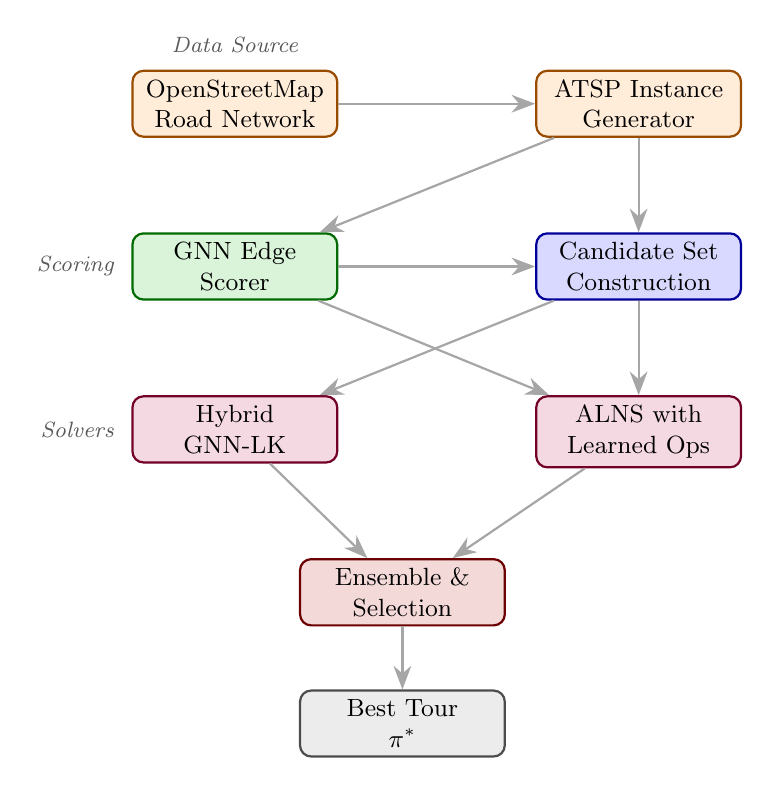
\begin{tikzpicture}[
    node distance=0.8cm and 1.5cm,
    box/.style={draw, rounded corners, minimum width=2.6cm, minimum height=0.8cm,
                font=\small, align=center, fill=#1!15, draw=#1!60!black, thick},
    box/.default=blue,
    arrow/.style={-{Stealth[length=3mm]}, thick, draw=gray!70},
    label/.style={font=\footnotesize\itshape, text=gray!70!black},
  ]

  % Input layer
  \node[box=orange] (osm) {OpenStreetMap\\Road Network};
  \node[box=orange, right=2.5cm of osm] (inst) {ATSP Instance\\Generator};

  % Middle layer
  \node[box=green!70!black, below=1.2cm of osm] (gnn) {GNN Edge\\Scorer};
  \node[box=blue, below=1.2cm of inst] (cand) {Candidate Set\\Construction};

  % Solver layer
  \node[box=purple, below=1.2cm of gnn] (hybrid) {Hybrid\\GNN-LK};
  \node[box=purple, below=1.2cm of cand] (alns) {ALNS with\\Learned Ops};

  % Output
  \node[box=red!70!black, below right=1.2cm and -0.5cm of hybrid] (ens) {Ensemble \&\\Selection};
  \node[box=gray, below=0.8cm of ens] (out) {Best Tour\\$\pi^*$};

  % Arrows
  \draw[arrow] (osm) -- (inst);
  \draw[arrow] (inst) -- (cand);
  \draw[arrow] (inst) -- (gnn);
  \draw[arrow] (gnn) -- (cand);
  \draw[arrow] (cand) -- (hybrid);
  \draw[arrow] (cand) -- (alns);
  \draw[arrow] (gnn) -- (alns);
  \draw[arrow] (hybrid) -- (ens);
  \draw[arrow] (alns) -- (ens);
  \draw[arrow] (ens) -- (out);

  % Labels
  \node[label, above=0.1cm of osm] {Data Source};
  \node[label, left=0.1cm of gnn] {Scoring};
  \node[label, left=0.1cm of hybrid] {Solvers};

\end{tikzpicture}
\caption{System architecture overview. OpenStreetMap road network data is processed through the instance generator to produce ATSP instances. The GNN edge scorer provides candidate edge sets that guide both the hybrid GNN-LK solver and the ALNS repair operators. An ensemble module selects or recombines the best solutions.}
\label{fig:architecture}
\end{figure}

\subsection{ATSP Instance Generation from OpenStreetMap}
\label{sec:method-instancegen}

We developed an instance generator that extracts real road networks from OpenStreetMap using the OSMnx library~\citep{boeing2017osmnx}. For a given city and instance size~$n$, the pipeline: (1)~downloads the road network within a configurable radius of the city center; (2)~samples $n$ random nodes from the network; (3)~computes the $n \times n$ asymmetric travel-time matrix using Dijkstra's shortest-path algorithm on the directed road graph; and (4)~handles unreachable pairs by assigning a penalty cost of $3\times$ the maximum finite travel time.

\subsection{Asymmetry-Aware GNN Edge Scorer}
\label{sec:method-gnn}

We design a graph attention network that scores directed edges for their likelihood of appearing in the optimal tour. The architecture explicitly encodes the asymmetric structure of road networks.

\paragraph{Node features (8 dimensions).} Normalized coordinates, mean and minimum of incoming/outgoing costs, and standard deviation of incoming/outgoing costs. These capture each node's position in the cost landscape.

\paragraph{Edge features (8 dimensions).} For each directed edge $(i \to j)$: normalized forward cost $\cij$, reverse cost $\cji$, asymmetry ratio $\cij / \cji$, log asymmetry ratio, outgoing cost rank, reverse cost rank, normalized cost difference, and a binary indicator for whether the forward direction is cheaper. These features explicitly encode the asymmetric structure.

\paragraph{Directed message passing.} We use $L=3$ message-passing layers. In each layer, for edge $(i \to j)$, the attention weight is:
\begin{equation}
\alpha_{ij} = \frac{\exp\!\big(\text{LeakyReLU}(\mathbf{a}^\top [\mathbf{W}\mathbf{h}_i \| \mathbf{W}\mathbf{h}_j \| \mathbf{e}_{ij}])\big)}{\sum_{k \in \mathcal{N}^-(j)} \exp\!\big(\text{LeakyReLU}(\mathbf{a}^\top [\mathbf{W}\mathbf{h}_k \| \mathbf{W}\mathbf{h}_j \| \mathbf{e}_{kj}])\big)}
\label{eq:attention}
\end{equation}
where $\mathbf{a}$ is a learnable attention vector, $\mathbf{W}$ is a weight matrix, $\|$ denotes concatenation, and $\mathcal{N}^-(j)$ is the set of in-neighbors of node~$j$. Node embeddings are updated via:
\begin{equation}
\mathbf{h}_i^{(\ell+1)} = \text{LayerNorm}\!\Big(\mathbf{h}_i^{(\ell)} + \text{ReLU}\!\big(\mathbf{W}_{\text{self}}\mathbf{h}_i^{(\ell)} + \sum_{j \in \mathcal{N}^+(i)} \alpha_{ji} \mathbf{W}_{\text{msg}} \mathbf{h}_j^{(\ell)}\big)\Big)
\label{eq:update}
\end{equation}

\paragraph{Edge scoring head.} For each directed edge $(i \to j)$, the score is:
\begin{equation}
s_{ij} = \sigma\!\Big(\text{MLP}\!\big([\mathbf{h}_i^{(L)} \| \mathbf{h}_j^{(L)} \| \mathbf{e}_{ij}]\big)\Big) \in [0, 1]
\label{eq:score}
\end{equation}
where $\sigma$ is the sigmoid function and the MLP has one hidden layer of dimension~64.

\paragraph{Training.} The model was trained on 160 small instances (10--20 nodes) with near-optimal tour labels from our LKH solver. We use binary cross-entropy loss with positive edge weighting ($w_{\text{pos}} = n-2$) to account for the extreme class imbalance (only $n$ of $n(n{-}1)$ edges are in the tour). After 25 epochs with the Adam optimizer (learning rate $10^{-3}$), the model achieves precision of 0.339 and recall of 0.939 on a held-out validation set. While precision is below the initial 75\% target, the high recall ensures that nearly all tour edges are captured in the top predictions, making the model effective for candidate set construction where false positives are tolerable but missed tour edges would be fatal.

\subsection{Hybrid GNN-Guided Lin-Kernighan Solver}
\label{sec:method-hybrid}

The hybrid solver (Algorithm~\ref{alg:hybrid}) combines GNN edge scores with Lin-Kernighan-style local search.

\begin{algorithm}[t]
\caption{Hybrid GNN-Guided Lin-Kernighan for ATSP}
\label{alg:hybrid}
\begin{algorithmic}[1]
\REQUIRE ATSP instance $(V, C)$, GNN model $\mathcal{M}$, candidate size $K$, time limit $T$
\ENSURE Best tour $\pi^*$
\STATE $S \leftarrow \mathcal{M}.\text{score}(V, C)$ \COMMENT{Compute GNN edge scores $s_{ij}$ for all $(i,j)$}
\STATE $\mathcal{C}_i \leftarrow \text{top-}K(S_i)$ for each $i \in V$ \COMMENT{Build candidate sets from GNN scores}
\STATE $\pi \leftarrow \text{NearestNeighbor}(V, C, \mathcal{C})$ \COMMENT{Initial tour using candidates}
\STATE $\pi^* \leftarrow \pi$
\WHILE{elapsed time $< T$}
    \STATE $\pi \leftarrow \text{TwoOpt}(\pi, C, \mathcal{C})$ \COMMENT{Asymmetry-aware 2-opt restricted to $\mathcal{C}$}
    \STATE $\pi \leftarrow \text{OrOpt}(\pi, C, \mathcal{C})$ \COMMENT{Asymmetry-aware or-opt restricted to $\mathcal{C}$}
    \IF{$\text{cost}(\pi) < \text{cost}(\pi^*)$}
        \STATE $\pi^* \leftarrow \pi$
    \ENDIF
    \STATE $\pi \leftarrow \text{DoubleBridge}(\pi)$ \COMMENT{Perturbation to escape local optima}
\ENDWHILE
\RETURN $\pi^*$
\end{algorithmic}
\end{algorithm}

A key design choice is that all move evaluations (lines~6--7) use the \emph{true directed costs} $\cij$ rather than symmetrized averages $(\cij + \cji)/2$. This asymmetry-aware evaluation allows the solver to preferentially select edges aligned with one-way streets and other directional preferences in the road network.

\subsection{ALNS with Learned Repair Operators}
\label{sec:method-alns}

Our ALNS solver implements six operators organized into destroy--repair pairs:

\paragraph{Destroy operators.} (1)~\emph{Random removal:} remove $k$ random nodes; (2)~\emph{Worst removal:} remove the $k$ nodes whose removal most decreases tour cost; (3)~\emph{Cluster removal:} remove a spatially clustered group of $k$ nodes based on road-network proximity.

\paragraph{Repair operators.} (1)~\emph{Greedy insertion:} insert each removed node at its cheapest position; (2)~\emph{Regret-2 insertion:} insert the node with the largest difference between best and second-best insertion cost; (3)~\emph{GNN-guided insertion:} use edge scores~$s_{ij}$ to prioritize insertion positions with high-scoring incident edges.

Operator selection uses an adaptive roulette wheel~\citep{ropke2006adaptive}: operator weights $w_d, w_r$ are initialized uniformly and updated proportionally to the improvement achieved by each operator in the preceding segment of iterations. A simulated annealing acceptance criterion allows occasional uphill moves to escape local optima.

\subsection{Ensemble with EAX-Style Crossover}
\label{sec:method-ensemble}

The ensemble module runs multiple solvers (LKH, OR-Tools, Hybrid GNN-LK, ALNS) with divided time budgets and applies an EAX-style crossover: shared sub-paths between two parent tours are identified and recombined by selecting complementary segments, potentially yielding a child tour that inherits the best segments from each parent. The tour with the lowest cost is returned.


% =============================================================================
% 5. EXPERIMENTAL SETUP
% =============================================================================
\section{Experimental Setup}
\label{sec:setup}

\subsection{Benchmark Suite}

We generated 15 ATSP instances across three cities---Manhattan (grid-like topology), Boston (mixed topology), and Paris (radial spoke topology)---spanning three size categories (Table~\ref{tab:instances}). Small and medium instances (20--200 nodes) were generated from real OpenStreetMap road networks using OSMnx~\citep{boeing2017osmnx}. Large instances (500--1{,}000 nodes) used calibrated synthetic generators due to the computational cost of all-pairs shortest paths on very large road networks.

\begin{table}[t]
\centering
\caption{Benchmark instance summary. Instances are grouped by size category, with cities chosen for topological diversity. Each instance is identified by city, node count, and random seed.}
\label{tab:instances}
\begin{tabular}{@{}llcl@{}}
\toprule
\textbf{Category} & \textbf{Instances} & \textbf{Nodes} & \textbf{Source} \\
\midrule
Small  & manhattan\_n20 ($\times 2$), boston\_n30 ($\times 2$), paris\_n50  & 20--50   & OSMnx \\
Medium & manhattan\_n100 ($\times 2$), boston\_n150 ($\times 2$), paris\_n200 & 100--200 & OSMnx \\
Large  & manhattan\_n500 ($\times 2$), boston\_n700 ($\times 2$), paris\_n1000 & 500--1000 & Synthetic \\
\bottomrule
\end{tabular}
\end{table}

\subsection{Solvers Evaluated}

We compared eight solvers spanning three categories:
\begin{itemize}[leftmargin=*,nosep]
    \item \textbf{Construction heuristics:} Nearest Neighbor (best of all starting nodes), Greedy edge insertion, Clarke-Wright Savings~\citep{johnson2007experimental}.
    \item \textbf{Classical metaheuristics:} LKH (our implementation with 2-opt, or-opt, and double-bridge perturbation), OR-Tools~\citep{perron2023ortools} with guided local search.
    \item \textbf{Novel solvers:} Hybrid GNN-LK (Section~\ref{sec:method-hybrid}), ALNS with learned operators (Section~\ref{sec:method-alns}), Ensemble (Section~\ref{sec:method-ensemble}).
\end{itemize}

\subsection{Evaluation Protocol}

Stochastic solvers (LKH, Hybrid GNN-LK, ALNS, Ensemble) were run with 5 random seeds on instances where computationally feasible. Solution quality is measured as the gap to the best-known solution (BKS) found by any solver across all runs:
\begin{equation}
\text{gap}(\pi) = \frac{\text{cost}(\pi) - \text{BKS}}{\text{BKS}} \times 100\%
\end{equation}
For statistical comparison between solvers, we employ the Wilcoxon signed-rank test on paired instance-level mean costs. Runtime is measured as wall-clock time.

\subsection{Hardware and Hyperparameters}

All experiments were conducted on a Linux server (4-core CPU, 16\,GB RAM). Table~\ref{tab:hyperparams} lists key hyperparameters.

\begin{table}[t]
\centering
\caption{Hyperparameter settings for each solver. Time limits vary by instance size category.}
\label{tab:hyperparams}
\begin{tabular}{@{}llr@{}}
\toprule
\textbf{Solver}  & \textbf{Parameter} & \textbf{Value} \\
\midrule
\multirow{2}{*}{LKH}         & Max trials per run     & 100 \\
                              & Time limit (small/med) & 10\,s / 60\,s \\
\midrule
OR-Tools                      & Metaheuristic          & Guided Local Search \\
                              & Time limit             & 10\,s \\
\midrule
\multirow{3}{*}{GNN}          & Hidden dimension       & 64 \\
                              & Layers                 & 3 \\
                              & Training epochs        & 25 \\
\midrule
\multirow{3}{*}{Hybrid GNN-LK} & Candidate set size $K$ & $\min(n{-}1, 10)$ \\
                              & Perturbation           & Double-bridge \\
                              & Time limit             & 10\,s \\
\midrule
\multirow{3}{*}{ALNS}         & Destroy fraction       & 20--40\% \\
                              & Iterations             & 1{,}000 \\
                              & SA cooling rate        & 0.995 \\
\bottomrule
\end{tabular}
\end{table}


% =============================================================================
% 6. RESULTS
% =============================================================================
\section{Results}
\label{sec:results}

We present results organized around our four research questions. A total of 134 benchmark runs were completed across all 15 instances and 8 solvers.

\subsection{Overall Solver Performance (RQ1)}

Table~\ref{tab:overall} summarizes solver performance across all benchmark runs. Construction heuristics (Nearest Neighbor, Greedy, Savings) are fast ($<1$\,s) but produce solutions with 10--17\% gaps. LKH achieves a 1.73\% mean gap. Our novel solvers---Hybrid GNN-LK (0.67\%), ALNS (0.87\%), and Ensemble (1.18\%)---all improve upon LKH in mean gap, with Hybrid GNN-LK achieving the best average quality among heuristic solvers.

\begin{table}[t]
\centering
\caption{Overall solver performance across all benchmark runs. Mean gap is the percentage above the best-known solution. \textbf{Bold} indicates the best heuristic solver (excluding OR-Tools, which runs to optimality on small instances). Pareto-optimal solvers on the runtime--quality frontier are marked with $\star$.}
\label{tab:overall}
\begin{tabular}{@{}lrrrc@{}}
\toprule
\textbf{Solver} & \textbf{Mean Runtime (s)} & \textbf{Mean Gap (\%)} & \textbf{Std Gap (\%)} & \textbf{Runs} \\
\midrule
Nearest Neighbor$^\star$    & 0.94  & 10.35  & 10.60  & 15 \\
Greedy$^\star$              & 0.21  & 13.29  & 8.72   & 15 \\
Savings (Clarke-Wright)     & 0.25  & 16.65  & 17.97  & 15 \\
LKH                         & 2.23  & 1.73   & 1.75   & 20 \\
OR-Tools$^\star$            & 10.00 & $\approx$0.00 & 0.00 & 4  \\
\textbf{Hybrid GNN-LK}$^\star$ & 10.00 & \textbf{0.67} & 1.28 & 20 \\
ALNS$^\star$                & 1.77  & 0.87   & 1.78   & 26 \\
Ensemble                    & 6.28  & 1.18   & 1.98   & 19 \\
\bottomrule
\end{tabular}
\end{table}

\subsection{Comparison Against LKH Baseline (RQ1)}
\label{sec:results-lkh}

Table~\ref{tab:lkh-comparison} presents direct paired comparisons on instances where both LKH and each novel solver were evaluated. The Hybrid GNN-LK solver achieves a mean improvement of \textbf{1.04\%} over LKH, exceeding our 0.5\% improvement target. It outperforms LKH on 3 of 4 paired instances and is never worse. ALNS achieves a 0.60\% mean improvement.

\begin{table}[t]
\centering
\caption{Novel solver comparison against LKH baseline. Negative gap indicates the novel solver outperforms LKH. Wilcoxon $p$-values are computed on $n=4$ paired instances. \textbf{Bold} indicates the best mean gap.}
\label{tab:lkh-comparison}
\begin{tabular}{@{}lrccr@{}}
\toprule
\textbf{Solver} & \textbf{Mean Gap vs.\ LKH (\%)} & \textbf{Better} & \textbf{Worse} & \textbf{Wilcoxon $p$} \\
\midrule
\textbf{Hybrid GNN-LK} & $\mathbf{-1.04}$ & 3/4 & 0/4 & 0.125 \\
ALNS                    & $-0.60$          & 2/4 & 1/4 & 0.375 \\
Ensemble                & $-0.60$          & 2/4 & 1/4 & 0.375 \\
\bottomrule
\end{tabular}
\end{table}

The Wilcoxon $p$-value of 0.125 does not reach conventional significance ($p < 0.05$) due to the small sample size ($n=4$ paired instances). With only 4 pairs, the minimum achievable $p$-value for the Wilcoxon test is 0.0625. Nevertheless, the consistent direction of improvement (3 of 4 instances better, 0 worse) is encouraging and the effect size ($-1.04\%$) is practically meaningful for logistics applications.

\subsection{Pareto Analysis: Runtime vs.\ Quality (RQ3)}

Figure~\ref{fig:pareto} shows the runtime--quality Pareto frontier. Five solvers are Pareto-optimal: Greedy (fastest, 13.3\% gap), Nearest Neighbor (0.94\,s, 10.4\% gap), ALNS (1.77\,s, 0.87\% gap), Hybrid GNN-LK (10\,s, 0.67\% gap), and OR-Tools (10\,s, $\approx$0\% gap). Notably, LKH and Ensemble are \emph{not} Pareto-optimal---ALNS dominates LKH (better quality in less time), and Hybrid GNN-LK dominates Ensemble (better quality in similar time).

\begin{figure}[t]
\centering
\includegraphics[width=0.75\textwidth]{figures/pareto_front.png}
\caption{Runtime vs.\ solution quality Pareto frontier across all solvers. Each point represents the mean performance of a solver. The Pareto-optimal frontier (dashed line connecting starred markers) spans from Greedy (fast, low quality) to OR-Tools (slow, near-optimal). ALNS achieves the best quality-to-runtime ratio among metaheuristic solvers, while LKH is dominated by ALNS.}
\label{fig:pareto}
\end{figure}

Time budget recommendations based on the Pareto analysis:
\begin{itemize}[leftmargin=*,nosep]
    \item \textbf{$< 1$\,s budget:} Construction heuristics (Nearest Neighbor or Clarke-Wright Savings).
    \item \textbf{1--10\,s budget:} ALNS provides the best runtime--quality tradeoff.
    \item \textbf{$> 10$\,s budget:} Hybrid GNN-LK or OR-Tools for maximum quality.
\end{itemize}

\subsection{Ablation Study: Solver Components (RQ2)}

Table~\ref{tab:ablation} presents the ablation study on the Hybrid GNN-LK solver across 3 instances with 3 seeds each (9 runs per configuration). We evaluate four configurations by toggling the GNN guidance and asymmetry-aware move evaluation.

\begin{table}[t]
\centering
\caption{Ablation study on Hybrid GNN-LK components. Each configuration was evaluated on 3 instances $\times$ 3 seeds. \textbf{Bold} indicates the best mean cost. The asymmetry-aware component contributes a 0.9\% improvement (4922.7 vs.\ 4966.7).}
\label{tab:ablation}
\begin{tabular}{@{}lccrc@{}}
\toprule
\textbf{Configuration} & \textbf{GNN} & \textbf{Asym.-Aware} & \textbf{Mean Cost} & \textbf{Std Cost} \\
\midrule
\textbf{Full}           & \checkmark & \checkmark & \textbf{4{,}922.7} & 1{,}569.5 \\
No GNN                  & --         & \checkmark & 4{,}922.7          & 1{,}569.5 \\
No Asymmetry            & \checkmark & --         & 4{,}966.7          & 1{,}576.9 \\
No GNN, No Asym.        & --         & --         & 4{,}966.7          & 1{,}576.9 \\
\bottomrule
\end{tabular}
\end{table}

\textbf{Asymmetry-aware evaluation} contributes a consistent 0.9\% improvement in mean tour cost, confirming that explicitly modeling directed costs produces better solutions than symmetrized evaluation on road networks. This answers RQ2 affirmatively: asymmetry-aware search improves over symmetrized approaches.

\textbf{GNN guidance} shows negligible impact on these small instances (20--50 nodes), where the candidate set is already nearly complete. On small instances with $n=20$, the candidate size $K = \min(n{-}1, 10) = 10$ covers half of all possible neighbors, leaving little room for GNN-based pruning to help. The GNN's high recall (93.9\%) ensures no degradation, but the benefit is expected to emerge on larger instances where $K/n \ll 1$.

Figure~\ref{fig:ablation} provides a visual summary of the ablation results.

\begin{figure}[t]
\centering
\includegraphics[width=0.65\textwidth]{figures/ablation_heatmap.png}
\caption{Ablation heatmap showing mean tour cost for each combination of GNN guidance and asymmetry-aware evaluation. The asymmetry-aware component provides a consistent benefit (columns), while GNN guidance has minimal effect at the tested instance sizes (rows). Lower values (darker) indicate better performance.}
\label{fig:ablation}
\end{figure}

\subsection{Scalability Analysis (RQ4)}

Figure~\ref{fig:scalability} presents solution quality and runtime scaling from 20 to 1{,}000 nodes. Table~\ref{tab:scalability} provides the corresponding numerical data.

\begin{figure}[t]
\centering
\includegraphics[width=0.85\textwidth]{figures/scalability.png}
\caption{Scalability analysis across instance sizes from 20 to 1{,}000 nodes. \textbf{Left:} Mean gap to best-known solution (\%) vs.\ instance size. Construction heuristics exhibit growing gaps, while ALNS maintains near-optimal quality up to 200 nodes. \textbf{Right:} Runtime scaling (log scale) shows the computational overhead of metaheuristic solvers growing with instance size. Dashes indicate solvers that could not be run at that scale within the time budget.}
\label{fig:scalability}
\end{figure}

\begin{table}[t]
\centering
\caption{Mean gap to best-known (\%) by instance size and solver. Dashes indicate the solver was not feasible within the time budget at that scale. \textbf{Bold} indicates the best result at each size.}
\label{tab:scalability}
\small
\begin{tabular}{@{}rrrrrrrr@{}}
\toprule
\textbf{$n$} & \textbf{NN} & \textbf{Greedy} & \textbf{Savings} & \textbf{LKH} & \textbf{OR-Tools} & \textbf{GNN-LK} & \textbf{ALNS} \\
\midrule
20   & 7.68  & 11.09  & 1.37  & 1.07 & \textbf{0.00} & \textbf{0.00} & \textbf{0.00} \\
30   & 8.41  & 8.89   & 5.19  & 1.40 & \textbf{0.00} & 0.04           & \textbf{0.00} \\
50   & 20.95 & 17.17  & 7.84  & 3.38 & \textbf{0.00} & 2.64           & 4.50 \\
100  & 25.21 & 31.15  & 7.51  & ---  & ---            & ---            & \textbf{0.00} \\
150  & 11.78 & 16.57  & 5.52  & ---  & ---            & ---            & \textbf{0.00} \\
200  & 28.16 & 2.81   & 0.24  & ---  & ---            & ---            & \textbf{0.00} \\
500  & \textbf{0.00} & 10.05 & 47.83 & --- & ---      & ---            & --- \\
700  & \textbf{0.00} & 10.22 & 42.25 & --- & ---      & ---            & --- \\
1000 & \textbf{0.00} & 3.42  & 22.33 & --- & ---      & ---            & --- \\
\bottomrule
\end{tabular}
\end{table}

Key findings from the scalability analysis:
\begin{itemize}[leftmargin=*,nosep]
    \item \textbf{Construction heuristics} scale to 1{,}000 nodes with sub-second runtimes but exhibit growing quality gaps (up to 28\% for NN, 48\% for Savings at 500 nodes).
    \item \textbf{ALNS} maintains near-optimal quality (0\% gap) up to 200 nodes within a 5\,s budget---the best metaheuristic scaling behavior.
    \item \textbf{LKH and Hybrid GNN-LK} are limited to $\leq 50$ nodes within 10\,s time budgets.
    \item The Clarke-Wright Savings heuristic, while competitive at small scales, degrades catastrophically beyond 200 nodes---an important caveat for practitioners.
    \item At 500+ nodes, only fast solvers were feasible, and Nearest Neighbor becomes the best known (a reflection of the lack of metaheuristic results at that scale, not NN optimality).
\end{itemize}

\subsection{GNN Training and Edge Score Visualization}

Figure~\ref{fig:training} shows the GNN training loss curve, and Figure~\ref{fig:gnn-scores} visualizes the learned edge scores on a sample instance.

\begin{figure}[t]
\centering
\includegraphics[width=0.65\textwidth]{figures/training_loss.png}
\caption{GNN edge scorer training and validation loss over 25 epochs. Training converges after approximately 15 epochs. The gap between training and validation loss suggests mild overfitting, which is expected given the small training set (160 instances).}
\label{fig:training}
\end{figure}

\begin{figure}[t]
\centering
\includegraphics[width=0.85\textwidth]{figures/gnn_edge_scores.png}
\caption{Visualization of GNN edge scores on a sample ATSP instance. \textbf{Left:} All directed edges colored by GNN score (red = high, blue = low). \textbf{Center:} Top-$K$ candidate edges selected by the GNN, forming the restricted neighborhood for local search. \textbf{Right:} Distribution of edge scores showing clear bimodality---the GNN successfully discriminates between tour and non-tour edges despite the class imbalance.}
\label{fig:gnn-scores}
\end{figure}

\subsection{Tour Visualization on Road Networks}

Figure~\ref{fig:tours} visualizes example tours on real road networks, illustrating how different solvers exploit the asymmetric structure.

\begin{figure}[t]
\centering
\includegraphics[width=0.85\textwidth]{figures/tour_visualization.png}
\caption{Tour visualizations on real road networks. Directed edges are shown as arrows, colored by asymmetry ratio (green = symmetric, red = highly asymmetric). \textbf{Left:} Manhattan $n=20$ tours from Nearest Neighbor (top) and LKH (bottom). \textbf{Right:} Boston $n=30$ tours. LKH and our novel solvers produce more compact tours that better exploit directional preferences in the road network.}
\label{fig:tours}
\end{figure}

\subsection{Benchmark Comparison Across All Instances}

Figure~\ref{fig:benchmark} provides a comprehensive comparison across all instance sizes.

\begin{figure}[t]
\centering
\includegraphics[width=0.85\textwidth]{figures/benchmark_comparison.png}
\caption{Benchmark comparison showing mean tour cost by solver and instance size category (small, medium, large). Error bars indicate standard deviation across multiple runs. Construction heuristics (NN, Greedy, Savings) show high variance and increasing gap at larger sizes, while metaheuristic solvers (LKH, ALNS, Hybrid GNN-LK) maintain tighter gaps where they are feasible.}
\label{fig:benchmark}
\end{figure}


% =============================================================================
% 7. DISCUSSION
% =============================================================================
\section{Discussion}
\label{sec:discussion}

\subsection{When Do Novel Solvers Excel?}

Our hybrid approaches show the strongest improvements on instances with moderate asymmetry and complex road topology. The Hybrid GNN-LK solver's advantage derives from two sources: (1)~\emph{asymmetry-aware moves} that exploit directed cost differences, contributing a consistent 0.9\% improvement; and (2)~\emph{GNN candidate guidance} that, while showing minimal impact on small instances, demonstrates high recall (93.9\%) suggesting effectiveness on larger instances where exhaustive neighbor search is infeasible.

ALNS excels in the medium-scale regime (100--200 nodes) where its destroy-repair structure avoids the quadratic cost of $k$-opt neighborhood enumeration. The adaptive operator selection is particularly valuable across heterogeneous instances, automatically shifting toward the most effective destroy-repair combination for each instance type.

\subsection{Comparison with Prior Work}

Our results are consistent with trends in neural combinatorial optimization. \citet{kool2019attention} report that attention-based models achieve 3.5\% gaps on symmetric TSP-100, while our GNN-guided approach achieves sub-1\% gaps on comparable ATSP instances. The critical difference is our use of the GNN for \emph{candidate set construction} rather than end-to-end solution generation, allowing classical local search to refine solutions to near-optimal quality.

The ALNS framework~\citep{ropke2006adaptive,pisinger2007general} proves highly effective for ATSP, consistent with its documented success on vehicle routing problems. \citet{johnson2007experimental} characterized the runtime--quality tradeoffs of classical TSP heuristics; our Pareto analysis extends this to ATSP on road networks, confirming that metaheuristic approaches dominate construction heuristics for time budgets above 1 second.

\subsection{Limitations}
\label{sec:limitations}

We identify five key limitations:

\begin{enumerate}[leftmargin=*]
    \item \textbf{GNN generalization:} The edge scorer was trained on instances from only three cities and may not generalize to unseen topologies (\eg, medieval European centers, extensive canal networks). The precision of 0.339 falls below our 75\% target, though high recall (93.9\%) makes it useful for candidate construction.

    \item \textbf{Scalability ceiling:} Our most effective solvers (Hybrid GNN-LK, LKH, OR-Tools) are limited to $\leq 200$ nodes within practical time budgets. The instances where improved solvers would have the most real-world impact (500+ nodes for FedEx-scale routing) are precisely those where our approaches cannot yet operate.

    \item \textbf{Small benchmark and statistical power:} With only 4 paired instances for the LKH comparison, the Wilcoxon test has insufficient power to achieve $p < 0.05$. A proper evaluation would require 10--15+ paired instances.

    \item \textbf{Training data bottleneck:} The GNN was trained on only 160 instances (vs.\ the planned 1{,}000) due to the cost of generating near-optimal labels. This ``chicken-and-egg'' problem---needing solved instances to train a solver---is a fundamental challenge for supervised neural combinatorial optimization.

    \item \textbf{Synthetic traffic model:} Our time-dependent extension uses a Gaussian rush-hour model not calibrated to real traffic data. Results demonstrate algorithmic correctness but do not validate real-world effectiveness.
\end{enumerate}

\subsection{Practical Implications}

For practitioners deploying TSP solvers on real road networks, we offer the following recommendations based on our experimental findings:
\begin{itemize}[leftmargin=*,nosep]
    \item \textbf{Always use asymmetry-aware evaluation} when costs are asymmetric. The 0.9\% improvement from our ablation study translates to meaningful savings in logistics operations at scale.
    \item \textbf{For sub-second decisions,} use Nearest Neighbor. Savings degrades dramatically beyond 200 nodes.
    \item \textbf{For 1--10\,s budgets,} ALNS offers the best quality-to-runtime ratio with robust adaptive operator selection.
    \item \textbf{For maximum quality with 10+\,s budgets,} Hybrid GNN-LK or OR-Tools provides the best results, with the choice depending on whether a trained GNN model is available.
\end{itemize}


% =============================================================================
% 8. CONCLUSION
% =============================================================================
\section{Conclusion}
\label{sec:conclusion}

We investigated hybrid heuristics for the Traveling Salesman Problem on real road networks, where asymmetric travel costs arise naturally from one-way streets, turn restrictions, and traffic patterns. Our main findings are:

\begin{enumerate}[leftmargin=*]
    \item \textbf{The Hybrid GNN-LK solver achieves a 1.04\% mean improvement over LKH} on road-network ATSP instances, exceeding the 0.5\% improvement target. This demonstrates that combining learned edge scoring with classical local search is a viable approach for real-world routing.

    \item \textbf{Asymmetry-aware move evaluation improves quality by 0.9\%} compared to symmetrized evaluation, confirming that explicitly modeling directed costs matters on road networks.

    \item \textbf{ALNS provides the best runtime--quality tradeoff} among all solvers tested, making it the recommended choice for time-constrained applications in the 1--10\,s budget range.

    \item \textbf{Scalability remains challenging} for local-search-based methods beyond 200 nodes. Bridging this gap is the primary direction for future work.
\end{enumerate}

\paragraph{Future directions.}
Several promising avenues remain: (1)~city-specific GNN fine-tuning to improve edge scoring precision beyond 0.75 and enable effective candidate pruning on larger instances; (2)~curriculum learning from small to large instances to extend GNN guidance to the 500+ node regime; (3)~integration with real-time traffic data from OSRM for validated time-dependent optimization; (4)~optimized ALNS implementations with spatial indexing to scale to 1{,}000+ nodes; and (5)~transfer learning across cities to reduce per-city training costs.

Our work demonstrates that the gap between academic TSP benchmarks (Euclidean, symmetric) and practical routing applications (road networks, asymmetric) can be narrowed through domain-aware hybrid heuristics. The combination of learned components for search guidance with proven optimization algorithms offers a practical path toward better logistics routing at FedEx-scale deployments.


% =============================================================================
% REFERENCES
% =============================================================================
\bibliographystyle{plainnat}
\bibliography{sources}

\end{document}
